\documentclass{sig-alternative}
% \documentclass[conference]{IEEEtran}
\usepackage{multirow}
\usepackage{color}
\usepackage{graphics} 
\usepackage{cite}
\usepackage{rotating}
\usepackage{eqparbox}
\usepackage{graphics}
\usepackage{colortbl} 
\usepackage{times}
\usepackage{balance}
\usepackage{picture}
\usepackage{algorithm}
\usepackage{algorithmicx}
\usepackage{algpseudocode}
\usepackage[export]{adjustbox}
\renewcommand{\footnotesize}{\scriptsize}
\definecolor{lightgray}{gray}{0.8}
\definecolor{darkgray}{gray}{0.6}
\renewcommand{\algorithmicrequire}{\textbf{Input:}}
\renewcommand{\algorithmicensure}{\textbf{Output:}}
%%% graph
\newcommand{\crule}[3][darkgray]{\textcolor{#1}{\rule{#2}{#3}}}
%\newcommand{\rone}{\crule{1mm}{1.95mm}}
%\newcommand{\rtwo}{\crule{1mm}{1.95mm}\hspace{0.3pt}\crule{1mm}{1.95mm}}
%\newcommand{\rthree}{\crule{1mm}{1.95mm}\hspace{0.3pt}\crule{1mm}{1.95mm}\hspace{0.3pt}\crule{1mm}{1.95mm}}
%\newcommand{\rfour}{\crule{1mm}{1.95mm}\hspace{0.3pt}\crule{1mm}{1.95mm}\hspace{0.3pt}\crule{1mm}{1.95mm}\hspace{0.3pt}\crule{1mm}{1.95mm}} 
%\newcommand{\rfive}{\crule{1mm}{1.95mm}\hspace{0.3pt}\crule{1mm}{1.95mm}\hspace{0.3pt}\crule{1mm}{1.95mm}\hspace{0.3pt}\crule{1mm}{1.95mm}}
\newcommand{\quart}[3]{\begin{picture}(100,6)%1
{\color{black}\put(#3,3){\circle*{4}}\put(#1,3){\line(1,0){#2}}}\end{picture}}
\definecolor{Gray}{gray}{0.95}
\definecolor{LightGray}{gray}{0.975}
% \newcommand{\rone}{}
% \newcommand{\rtwo}{}
% \newcommand{\rthree}{}
% \newcommand{\rfour}{} 
% \newcommand{\rfive}{}
\newcommand{\wei}[1]{\textcolor{red}{Wei: #1}} 
\newcommand{\Menzies}[1]{\textcolor{red}{Dr.Menzies: #1}} 

%% timm tricks
\newcommand{\bi}{\begin{itemize}[leftmargin=0.4cm]}
\newcommand{\ei}{\end{itemize}}
\newcommand{\be}{\begin{enumerate}}
\newcommand{\ee}{\end{enumerate}}
\newcommand{\tion}[1]{\S\ref{sect:#1}}
\newcommand{\fig}[1]{Figure~\ref{fig:#1}}
\newcommand{\tab}[1]{Table ~\ref{tab:#1}}
\newcommand{\eq}[1]{Equation~\ref{eq:#1}}

%% space saving measures

\usepackage[shortlabels]{enumitem}  
\usepackage{url}
% \def\baselinestretch{1}


% \setlist{nosep}
%  \usepackage[font={small}]{caption, subfig}
% \setlength{\abovecaptionskip}{1ex}
%  \setlength{\belowcaptionskip}{1ex}

%  \setlength{\floatsep}{1ex}
%  \setlength{\textfloatsep}{1ex}
%  \newcommand{\subparagraph}{}

% \usepackage[compact,small]{titlesec}
% \DeclareMathSizes{7}{7}{7}{7} 
% \setlength{\columnsep}{7mm}

\begin{document}
% \conferenceinfo{FSE}{'15 Bergamo, Italy}
\title{ XYZ}
\numberofauthors{2}
\author{
        \alignauthor Vivek Nair, Tim Menzies, Xipeng Shen 
        \affaddr{Computer Science, North Carolina State University, Raleigh, USA}
        \email{vivekaxl, tim.menzies, xipengshen@gmail.com}
    \and  
        \alignauthor Norbert Siegmund, Sven Apel \\
        \affaddr{Computer Science, University of Passau, Germany}\\
        \email{norbert.siegmund, apel@uni-passau.de}
       }

\maketitle 
\thispagestyle{plain}
\pagestyle{plain}
\begin{abstract}
Active Learning, Configuration, Sampling, Machine Learning, Performance Prediction


\end{abstract}

% A category with the (minimum) three required fields
\vspace{1mm}
\noindent
{\bf Categories/Subject Descriptors:} 
D.2 [Software Engineering] ;
I.2.6 [Artificial Intelligence]: Induction

 
\vspace{1mm}
\noindent
{\bf Keywords:} Performance prediction, Active Learning, 
Multi-Objective Optimization,
Search-based Software Engineering,Sampling, Machine Learning.

\pagenumbering{arabic} %XXX delete before submission
 
 
\section{Introduction}
 
\bi
    \item{Challenges}
    \item{Solutions Proposed}
    \item{Research Questions}
\ei
\section{Bird's Eye Overview}
\bi
    \item{Sampling}
    \item{Fast Learners}
\ei

\section{Data U}
\section{Sampling Technique: East-West Where}
\bi
    \item{WHERE}
\ei
\section{Fast Searcher: GALE}





 

% \subsection{Data Mining Algorithms}
 
% There are many ways to build defect predictors
% such as  CART
% and WHERE
% For this study, we use the CART and Random Forest  from 
% SciKitLearn~
% WHERE is available from
% github.com/ai-se/where).
%  We use  these algorithms, for the following reasons.
% CART and Random Forest were mentioned in
% a recent IEEE TSE paper by Lessmann et al.~
% learners for  defect prediction.
% That study ranked  CART  worst  and Random Forest as best.
% In a demonstration of the impact of tuning,
% this paper shows  we can {\em reverse} the conclusions of  Lessmann et al. such that CART
% performs just as well as
%  Random Forest.
% This
%  paper also presents results with WHERE-based learner since, as shown below,
% it offers an interesting case study on the benefits of tuning.
  

% \subsection{Learners and Their Tunings}


% Our learners use the tuning parameters of \tab{parameters}. This section describes those parameters.

% As shown in \tab{parameters}, default parameters for the Where-based learner are set using authors' engineering judgment and default parameters for CART and Random Forests are set by SciKitLearn. Those default parameters might not be the standard parameters for practical defect learners in reality, but it's a rule of thumb that most researchers would use just use the default parameters in the software without any tuning


% CART, Random Forest, and WHERE-based learners are all  tree learners that divide a data set, then recur
% on each split.
% All these learners
% generate numeric predictions which are converted
% into binary ``yes/no'' decisions via \eq{yesno}.

% \begin{equation}\label{eq:yesno}\scriptsize
% \mathit{inspect}= \left\{
% \begin{array}{ll}
% d_i \ge T \rightarrow \mathit{Yes}\\
% d_i <   T \rightarrow \mathit{No} ,
% \end{array}\right.
% \end{equation}
% The splitting process is controlled by numerous tuning parameters.
% If data contains more than {\em min\_sample\_split}, then a split is attempted.
% On the other hand, if a split contains no more than {\em min\_samples\_leaf}, then recursion stops. CART and Random Forest use a 
% user-supplied constant for this parameter while
% WHERE-based learner firstly computes this parameter $m$={\em min\_samples\_leaf} from the size of the data
% sets via  $m=\mathit{size}^\mathit{min\_size}$ to build an initial  clustering tree.
% Note that WHERE builds {\em two} trees: the initial clustering tree (to find similar sets of data)
% then a final decision tree (to learn rules that predict for each similar cluster)\footnote{A
% frequently asked question is why does WHERE build two trees--
% would not   a single tree suffice? The answer is, as shown below,  tuned WHERE's twin-tree approach 
% generates very precise predictors.}.
% The tuning parameter  {\em min\_sample\_ split } controls the construction of the
% final decision tree (so, for WHERE-based learner,
% {\em min\_size} and {\em min\_sample\_split} are the parameters to be tuned).

% These learners use different techniques to explore the splits:
% \bi
% \item
% CART finds the attributes whose ranges contain rows with least variance in the number
% of defects\footnote{If an attribute ranges $r_i$ is found in 
% $n_i$ rows each with a  defect count variance of $v_i$, then CART seeks the attributes
% whose ranges minimizes $\sum_i \left(\sqrt{v_i}\times n_i/(\sum_i n_i)\right)$.}.
% \item
% Random Forest    divides data like CART then  builds $F>1$  trees,
% each time using some random subset of
% the attributes. 
% \item
% When building the initial cluster tree, WHERE projects the data on to a dimension it synthesizes from the raw data using
% a process analogous to principle component analysis\footnote{
% PCA  synthesises  new
% attributes $e_i, e_2,...$
% that extends across the dimension of greatest  variance in the data  with attributes $d$.  
% This process  combines
% redundant  variables into a smaller set of variables  (so $e \ll d$) since those
% redundancies become (approximately) parallel lines
% in $e$ space. For all such redundancies \mbox{$i,j \in d$}, we 
% can ignore $j$ 
% since effects that change over $j$ also
% change in the same way over $i$.
% PCA is also useful for skipping over noisy variables from $d$-- these
% variables are effectively ignored since    they  do not contribute to the variance in the data.}.
% WHERE  divides  at the median point of that projection.
% On recursion,
% this generates the initial clustering tree, the leaves of which are clusters of  very similar examples. After that, when building 
% the final decision tree, WHERE pretends its clusters are ``classes'', then 
% asks the InfoGain of the
% Fayyad-Irani discretizer~
% WHERE's final decision tree generator then ignores everything except the top   {\em infoPrune} percent of the sorted
% attributes.
% \ei
% Some tuning parameters are learner specific:
% \bi
% \item
% {\em Max\_feature} is used by
% CART and Random Forest to select the number of attributes
% used to build one tree.
% CART's default is to use all the attributes while 
% Random Forest usually selects the square root of the number
% of attributes.
% \item
%   {\em Max\_leaf\_nodes} is the upper bound on leaf notes generated in a 
%   Random Forest.
% \item {\em Max\_depth} is the upper bound on the depth of the CART tree.  
%  \item
% WHERE's initial clustering
% tree generation will always split up to {\em depthMin} number of branches.
% After that, WHERE will only split data if the mean performance scores of the two halves
% is ``trivially small'' (where ``trivially small'' is set by the   {\em wriggle} parameter). 
% \item
% WHERE's   {\em tree\_prune} setting controls how   
% WHERE prunes back superflous parts of the final decision tree. 
% If a decision sub-tree and its parent have the same 
% majority cluster
% (one that occurs most frequently), then if {\em tree\_prune} is enabled, we prune that decision sub-tree.
% \ei



% \subsection{Tuning Algorithms}


%  \subsubsection{Parametric Tuning Algorithms}
% The  goal of this paper is to adjust the tuning parameters of \tab{parameters}
% in order to   optimize (improve) some particular performance scores
% generated by a particular learner being applied to  a particular data set.
% For this task, we do not use traditional parametric numeric optimizer  
% such as  gradient descent optimizers~
% differential functions (i.e. functions of real-valued variables whose derivative exists at each point in its domain).
% This is impractical  for  our learners since their internal states are   not a smoothly differential continuous function.
% Rather, learners being tuned  contain many regions with many different properties (tuning options can
% drive the learner into very different modes with very different performance properties).


%  \subsubsection{Non-Parametric Tuning Algorithms}
 
% Non-parametric  optimizers   make no assumption
% about the internal structure of the model.
% There are many such optimizers:
% \bi
% \item
% Simulated annealing~
% \item
% A wide range of genetic algorithms~
% techniques such as differential evolution~
% \item
% Particle swarm optimization~
% \item 
% Numerous ``decomposition approaches'' that uses
%     heuristics to decompose the total space into   small problems,   then applies a
%     simpler optimizer to each region including \mbox{$\varepsilon$-domination}~
%     \item 
%     Response surface methods~
%     \item
%     And many others as well.
%     \ei
% From all the above methods, how do we select which optimizers to apply to tuning data miners?
% Cohen~
%  methods against the simplest possible alternative. 
% Holte~
%  as a
% kind of ``scout'' for a  preliminary analysis of a data
% set (to check if that data really requires a more
% complex analysis).

% To find our ``scout'',  we used engineering judgement to sort  the above algorithms from simplest to most complex.
% Of the optimizers listed above, the simplest are simulated annealing (SA)  and 
% differential evolution (DE), each of which can be coded in less than a page of some high-level scripting language. Our reading of the current literature is that there are more  advocates for
% differential evolution than
%   SA:
%   \bi
%   \item
%   When the MOEA/D community requires a secondary optimizer, they often use  differential evolution~
%   \item
%  Vesterstrom and Thomsen~
%   particle swarm optimization and other GAs.
%   \ei
% DEs have been applied before for   parameter tuning (e.g. see~
% optimize defect prediction from static code attributes.  
% The psuedocode for differential evolution is shown in Algorithm~\ref{alg:DE}.
% In the following description, 
%     superscript numbers denotes a line in that figure.
 
% \subsection{RQ2:  Does Tuning Change a Learner's Ranking Regarding Different Goals?}\label{sect:rank}
% Researchers often use performance criteria to assert that one learner is better than another~

% 22 learners are compared over NASA MDP data sets in terms of the AUC in 

% In \tab{precisionbars} and \tab{fbars}, the tuned CART are better than or equal to tuned Random Forests over $\frac{11}{17}$ and $\frac{10}{17}$ data sets in
% terms of precision and F-measure, respectively. Results from the non-parametric Kolmogorov-Smirnov Test turn out that the performance 
% scores of tuned CART and tuned Random Forests are not statistically different. This is the opposite of   
%  Lessmann et al.~
%  In another result that is the reverse of \tab{precisionbars}, tuned WHERE is not necessarily
%  any better than anything else.
 
%  Therefore, it's not always safe to say ``LearnerX'' is the best or better than ``learnerY'' without pointing out the performance criteria or applying tuning techniques. That is, the answer to RQ2 is ``yes'' since tuning a set of learners
%  changes the rankings of those learners regarding different criteria.
 
% The  important lesson here is that, given a particular task (e.g. optimizing for precision), tuning can offer
% substantial benefits. However, when that task changes (e.g. to optimizing for the F-measure),
% it should not be assumed that conclusions from the previous tuning will hold in the new context.
% In practice, this means that tuning needs to be repeated for each new context.


% % \begin{figure}[!t]
% % \begin{center}
% % 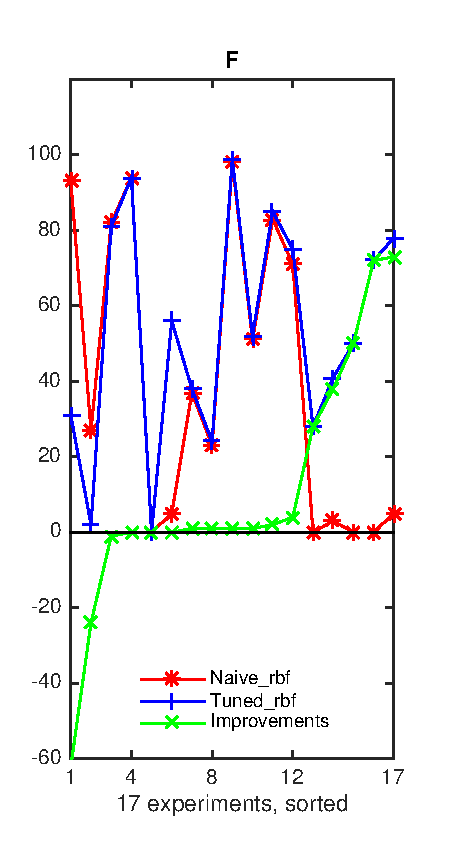
\includegraphics[width=1.5in]{svm_rbf.eps}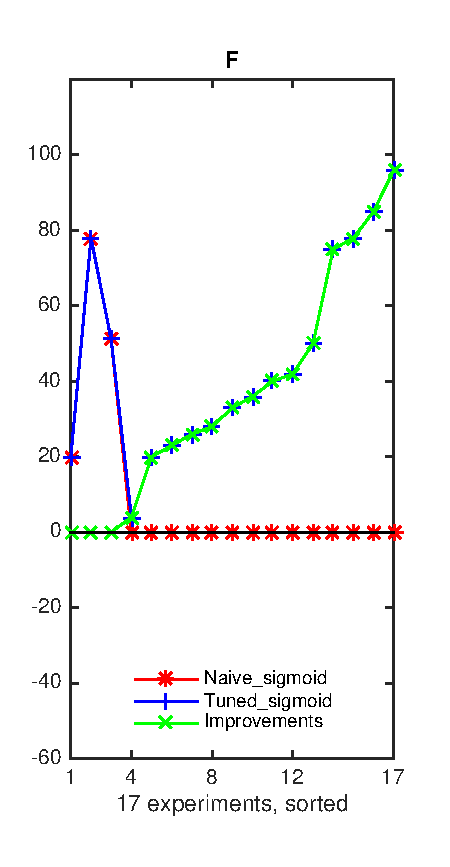
\includegraphics[width=1.5in]{svm_sigmoid.eps}
% %  \end{center}
% % \caption{Comparison between tuned and naive SVM learners with rbf and sigmoid kernels over the goal of F. }\label{fig:svm}
% %  \end{figure}

 
% \subsection{RQ4: Is Tuning Easy?}\label{sect:easy}

% In terms of the search space
% explored via tuning, optimizing defect prediction from static code
% measures is much {\em smaller} than the standard optimization.

% To see this,
% recall from Algorithm~1 that
% DE explores a {\em Population} of size {\em np=10}. This is a very small population size since
% Rainer Storn (one of the inventors of DE) recommends  setting {\em np} to be ten times larger than the number
% of attributes being optimized~

% From \tab{parameters},
% we see that Storn would therefore recommend {\em np} values of
% 90, 50, 60 for WHERE, CART and Random Forests (respectively). Yet we achieve our results
% using a constant {\em np=10}; i.e. $\frac{10}{90}, \frac{10}{50}, \frac{10}{60}$ of the
% recommended search space.

% To justify that {\em np=10} is enough, we did another tuning study, 
% where all the settings were the same as before but we set{\em np= 90, 50} and {\em np = 60} for WHERE, CART and Random Forests as recommended by Storn. The tuning performance of learners was evaluated
% by precision and F. To compare performance of each learner with different np's, we plot the delta in the performance as \fig{deltas}. As shown in \fig{deltas_np}, in terms of precision, the recommended {\em np} will improve the performance of WHERE, CART and Random Forests in 2, 5, and 4 data sets. However, in 6, 4, and 4 data sets, those numbers  will degrade the performance compared with {\em np = 10}. For F as the tuning goal, we can observe the similar pattern. 

%  From this study, with the same experimental condition, the recommended {\em np's} for WHERE, CART and Random Forest, do not bring any significant improvements over {\em np = 10}. We're not arguing that {\em np = 10} is the optimal settings for tuning defect predictors. But it suffices to make tuning easy and generate a competitive performance.

% Another measure showing that tuning is easy 
% (for static code defect predictors)
% is the number of evaluations required to complete optimization
% (see next section).

% Hence we answer RQ4 as ``yes'', tuning is surprisingly easy (at least
% for defect predictors).




% % %%% repalce this table with the new one
% % \begin{table}[!ht]

% % \renewcommand{\baselinestretch}{0.8}
% % \scriptsize
% % \centering
% %   \begin{tabular}{c|c c|c c|c c|c c| c c }
  
% %     &   \multicolumn{2}{c|}{Precision} & \multicolumn{2}{c|}{F} &  \multicolumn{2}{c|}{SUM}\\
% %  &&&&&&&\\
% % Features&   
% %   default
% % & tuned
% % & default
% % & tuned
% % & default
% % & tuned
% % \\\hline

% % max\_cc& & & &  & & \\
% % noc& & & & & & \\
% % ca& & & & & & \\
% % cbo& & 1& & & & 1\\
% % moa& & 1& & & & 1\\
% % ce& & 2& & 1& & 3\\
% % avg\_cc& & 2& & 2& & 4\\
% % npm& 1& 2& 1& 1&2 & 3\\
% % lcom& 1& 2& 1& 1& 2& 3\\
% % amc& 4& 2& 4& 2& 8& 4\\
% % cbm& 5& 2& 5& 3& 10& 5\\
% % rfc& 3& 6& 3& 8& 6& 14\\
% % wmc& 5& 4& 5& 9& 10& 13\\
% % dit& 8& 3& 7& 7& 15& 10\\
% % ic& 8& 3& 8& 6& 16 & 9\\
% % lcom3& 8& 6& 8& 8&16 & 14\\
% % cam& 9& 7& 9& 7& 18& 14\\
% % loc& 9& 5& 9& 11& 18& 16\\
% % dam& 13& 6& 13& 11& 26& 17 \\
% % mfa& 16& 9& 16& 9&32 & 18\\

 
% %   \end{tabular}
% %     \caption{Counts of features selected by different goals.Given that we are processing 17 data sets, the maximum counts for any 
% % one cell in the ``precision'' or ``F'' column is 17.  
% %     }\label{tab:counts}
% % \end{table}
  
% Hence, we answer RQ5 as ``no''. Tuning is so fast that
% it could (and should) be used by anyone using defect predictors. The possible reason that tuning is so fast is that the searching space for defect prediction is not complicated, which might result from the tuning range set for each parameter in \tab{parameters}. The early stopping rules applied in this study also helps make tuning fast

% \subsection{RQ6: Should we use ``off-the-shelf'' Tunings?}\label{sect:variance}
 
%  In \fig{features}, we show how tuning selects the optimal values for parameters. For space limitation, only four parameters from WHERE learner are selected as representative and all the others can be found in our supporting documents\footnote{\url{https://goo.gl/aHQKtU}}.
% The default value for {\em threshold}, {\em infoPrune}, {\em min\_Size} and {\em wriggle} are $0.5$, $0.33$, $0.5$ and $0.2$. Note that:
% \bi
% \item
% The tunings learned by DE
% were often very different to the default. That is, to achieve the performance improvements seen in the paper,
% the default tuning parameters required a wide range of adjustments.
% \item The tunings learned by DE were different in different data sets and for different goals.
% \ei
% Hence, we answer RQ6 as ``no'' since, to achieve the improvements seen in this paper, tuning has to be repeated whenever the goals or data
% sets are changed.Given this requirement to repeatedly run tuning, it is fortunate that (as shown above)
% tuning is so easy and so fast (at least for defect predictors from static code attributes). %%%%%
% \begin{table*}[!ht]
 
% \renewcommand{\baselinestretch}{0.9}
% \resizebox{\textwidth}{!}{
% \scriptsize
% \centering
%   \begin{tabular}{|c |c |c |c |c |c |c |c |c |c |c |c |c |c |c |c |c |c |c |c |}
%     \hline
%   \begin{tabular}[c]{@{}c@{}}Learner \\ Name\end{tabular}&Parameters  & Default &antV0&antV1&antV2&camelV0&camelV1&ivy&jeditV0&jeditV1&jeditV2&log4j&lucene&poiV0&poiV1&synapse&velocity&xercesV0&xercesV1\\ 
%  \hline
% \multirow{8}{*}{\begin{tabular}[c]{@{}c@{}}Where\\based\\ Learner\end{tabular}}
% & threshold& 0.5& 0.98& 0.98& 0.43& 0.24& 0.64& 1& 1& 0.98& 0.98& 1& 1& 0.87& 0.59& 0.98& 1& 0.98& 0.98\\ \cline{2-20}
% & infoPrune& 0.33& 0.05& 0.05& 0.71& 0.54& 0.45& 0.41& 0.3& 0.05& 0.05& 0.54& 0.84& 0.01& 1& 0.05& 0.68& 0.43& 0.05\\ \cline{2-20}
% & min\_sample\_size& 4& 7& 7& 9& 8& 6& 10& 1& 5& 7& 8& 7& 9& 3& 7& 7& 1& 7\\ \cline{2-20}
% & min\_Size& 0.5& 0.51& 0.51& 0.59& 0.46& 0.13& 0.38& 0.66& 0.27& 0.51& 0.46& 0.47& 0.77& 0.48& 0.51& 0.66& 0.22& 0.51\\ \cline{2-20}
% & wriggle& 0.2& 0.6& 0.6& 0.83& 0.52& 0.19& 0.01& 0.26& 0.6& 0.6& 0.52& 0.19& 0.83& 0.01& 0.6& 0.26& 0.55& 0.6\\ \cline{2-20}
% & depthMin& 2& 1& 1& 2& 3& 5& 2& 3& 3& 1& 1& 2& 4& 2& 1& 3& 2& 1\\ \cline{2-20}
% & depthMax& 10& 8& 8& 13& 19& 19& 18& 7& 8& 8& 19& 1& 19& 18& 8& 11& 18& 8\\ \cline{2-20}
% & wherePrune& False& False& False& False& False& True& True& False& False& False& False& False& True& True& False& False& True& False\\ \cline{2-20}
% & treePrune& True& False& False& False& True& True& True& False& False& False& True& True& False& False& False& False& True& False\\ \cline{2-20}
% \hline
% \multirow{4}{*}{CART}
% & threshold& 0.5& 0.69& 0.99& 1& 0.3& 0.83& 1& 0.99& 0.58& 0.72& 1& 0.71& 0.46& 0.72& 1& 0.85& 1& 0.64\\ \cline{2-20}
% & max\_feature& None& 0.01& 0.58& 0.65& 0.66& 0.73& 0.67& 0.56& 0.01& 0.97& 0.54& 0.52& 0.32& 0.01& 0.74& 0.73& 0.01& 0.1\\ \cline{2-20}
% & min\_samples\_split& 2& 7& 16& 18& 5& 11& 6& 15& 6& 17& 4& 16& 12& 5& 14& 11& 4& 10\\ \cline{2-20}
% & min\_samples\_leaf& 1& 13& 14& 10& 4& 3& 15& 16& 9& 6& 7& 6& 1& 4& 6& 7& 11& 7\\ \cline{2-20}
% & max\_depth& None& 14& 1& 41& 34& 1& 22& 29& 1& 1& 1& 14& 19& 8& 40& 4& 1& 1\\ \cline{2-20}
% \hline
% \multirow{6}{*}{\begin{tabular}[c]{@{}c@{}}Random \\ Forests\end{tabular}} 
% & threshold& 0.5& 0.84& 0.9& 0.83& 0.33& 1& 0.99& 0.91& 1& 1& 0.83& 0.98& 0.9& 0.86& 0.83& 1& 1& 1\\ \cline{2-20}
% & max\_feature& None& 0.61& 0.13& 0.89& 0.37& 0.01& 0.98& 0.52& 0.75& 0.35& 0.01& 0.98& 0.84& 0.73& 0.01& 0.48& 0.51& 0.01\\ \cline{2-20}
% & max\_leaf\_nodes& None& 37& 35& 38& 21& 36& 45& 10& 38& 10& 30& 20& 43& 11& 13& 15& 39& 10\\ \cline{2-20}
% & min\_samples\_split& 2& 8& 16& 17& 13& 14& 2& 3& 2& 2& 18& 19& 9& 4& 4& 9& 20& 1\\ \cline{2-20}
% & min\_samples\_leaf& 1& 19& 5& 2& 4& 2& 4& 7& 17& 7& 16& 12& 2& 3& 2& 2& 2& 3\\ \cline{2-20}
% & n\_estimators& 100& 138& 112& 77& 74& 125& 130& 107& 85& 96& 111& 103& 82& 59& 149& 150& 63& 58\\ \cline{2-20}
% \hline  \end{tabular}
% }
%   \caption{Parameters tuned on different models over the objective of precision.}\label{tab:preselect}
% \end{table*}


% %%%%parameters for F %%%%%%
% \begin{table*}[!ht]
 
% \resizebox{\textwidth}{!}{
% \renewcommand{\baselinestretch}{0.9}
% \scriptsize
% \centering
%   \begin{tabular}{|c |c |c |c |c |c |c |c |c |c |c |c |c |c |c |c |c |c |c |c |}
%     \hline
    
%   \begin{tabular}[c]{@{}c@{}}Learner \\ Name\end{tabular}&Parameters  & Default &antV0&antV1&antV2&camelV0&camelV1&ivy&jeditV0&jeditV1&jeditV2&log4j&lucene&poiV0&poiV1&synapse&velocity&xercesV0&xercesV1\\ 
%  \hline
% \multirow{8}{*}{\begin{tabular}[c]{@{}c@{}}Where\\based\\ Learner\end{tabular}}
% & threshold& 0.5& 0.04& 0.44& 0.44& 0.98& 0.65& 0.77& 1& 0.65& 0.98& 0.44& 0.44& 0.87& 0.04& 0.77& 0.24& 0.44& 0.77\\ \cline{2-20}
% & infoPrune& 0.33& 0.51& 0.68& 0.88& 0.47& 0.07& 0.31& 0.48& 0.68& 0.57& 0.12& 0.68& 0.01& 0.51& 0.14& 0.54& 0.68& 0.14\\ \cline{2-20}
% & min\_sample\_size& 4& 6& 4& 6& 1& 6& 8& 8& 4& 6& 7& 4& 9& 6& 2& 8& 4& 8\\ \cline{2-20}
% & min\_Size& 0.5& 0.18& 0.4& 0.56& 0.51& 0.65& 0.59& 0.97& 0.4& 0.51& 0.8& 0.4& 0.77& 0.18& 0.62& 0.46& 0.4& 0.66\\ \cline{2-20}
% & wriggle& 0.2& 0.25& 0.29& 0.76& 0.6& 0.63& 0.26& 1& 0.51& 0.17& 0.36& 0.51& 0.83& 0.25& 0.5& 0.52& 0.29& 0.26\\ \cline{2-20}
% & depthMin& 2& 3& 3& 3& 1& 5& 3& 2& 3& 5& 5& 3& 4& 3& 3& 3& 3& 3\\ \cline{2-20}
% & depthMax& 10& 16& 15& 15& 8& 19& 10& 7& 15& 5& 15& 15& 19& 16& 6& 19& 15& 10\\ \cline{2-20}
% & wherePrune& False& False& True& True& True& True& True& True& False& False& True& True& True& False& True& False& False& True\\ \cline{2-20}
% & treePrune& True& False& True& True& False& False& False& False& False& True& True& True& False& False& False& True& True& False\\ \cline{2-20}
% \hline
% \multirow{5}{*}{CART}
% & threshold& 0.5& 0.34& 0.25& 0.01& 0.01& 0.73& 0.53& 0.92& 0.8& 0.74& 0.54& 0.03& 0.91& 0.01& 0.01& 0.55& 1& 0.01\\ \cline{2-20}
% & max\_feature& None& 0.01& 0.01& 0.29& 0.01& 0.46& 0.75& 0.79& 0.74& 0.41& 0.81& 0.61& 0.72& 0.01& 0.01& 0.01& 0.25& 0.18\\ \cline{2-20}
% & min\_samples\_split& 2& 18& 20& 12& 2& 15& 11& 2& 18& 13& 9& 17& 16& 10& 4& 8& 3& 15\\ \cline{2-20}
% & min\_samples\_leaf& 1& 19& 16& 15& 17& 1& 1& 13& 10& 4& 3& 7& 5& 20& 7& 8& 1& 6\\ \cline{2-20}
% & max\_depth& None& 12& 2& 15& 1& 41& 20& 44& 15& 13& 5& 23& 14& 1& 5& 17& 47& 13\\ \cline{2-20}
% \hline
% \multirow{6}{*}{\begin{tabular}[c]{@{}c@{}}Random \\ Forests\end{tabular}} 
% & threshold& 0.5& 0.01& 0.35& 0.3& 0.01& 0.9& 0.97& 0.63& 1& 0.73& 0.68& 0.01& 1.0& 0.01& 0.07& 0.22& 1& 0.82\\ \cline{2-20}
% & max\_feature& None& 0.63& 0.17& 0.01& 0.01& 0.88& 0.74& 0.76& 0.73& 0.01& 0.03& 0.39& 0.02& 0.01& 0.56& 0.36& 0.51& 0.89\\ \cline{2-20}
% & max\_leaf\_nodes& None& 40& 33& 46& 22& 11& 16& 38& 34& 30& 31& 12& 49& 25& 47& 15& 39& 24\\ \cline{2-20}
% & min\_samples\_split& 2& 10& 16& 20& 1& 1& 1& 1& 4& 20& 19& 11& 14& 2& 17& 19& 20& 19\\ \cline{2-20}
% & min\_samples\_leaf& 1& 4& 15& 9& 13& 18& 11& 3& 16& 17& 6& 10& 7& 19& 13& 11& 2& 14\\ \cline{2-20}
% & n\_estimators& 100& 120& 73& 75& 130& 97& 144& 125& 97& 80& 111& 96& 101& 50& 67& 74& 63& 66\\ \cline{2-20}
% \hline  \end{tabular}
% }
%   \caption{Parameters tuned on different models over the objective of ``F''.}\label{tab:fselect}
% \end{table*}
 \begin{table*}[!h]
 
 \begin{tabular}{c c c c c c} 

 
 \hline
 Project & Domain & Lang. & LOC & Features & Configs \\  
 \hline
 Berkeley DB CE & Database & C & 219,811 & 18 & 2560  \\ 
 
 Berkeley DB JE & Database & Java & 42,596 & 32 & 400 \\

 Apache & Web Server & C & 230,277 & 9 & 192 \\

 SQLite & Database & C & 312,625 & 39 & 3,932,160 \\
 
 LLVM & Compiler & C++ & 47,549 & 11 & 1024 \\ 

 x264 & Video Enc. & C & 45,743 & 16 & 1152 \\ 

\end{tabular}
 \caption{Overview of the programs used in the evaluations}
\end{table*}


 \begin{table*}[!h]
 

 \begin{tabular}{c c } 
 \hline
 Project & Benchmark/Job Used  \\  
 \hline
 Berkeley DB CE & Vendor Provided  \\ 
 
 Berkeley DB JE & Vendor Provided \\

 Apache & autobench + httperf \\

 SQLite & Vendor Provided \\
 
 LLVM & opt-tools \\ 

 x264 & Sintel(735MB) \\
 

\label{BenchMarkUsed} 
\end{tabular}
\caption{Overview of the benchmarks used in the evaluations}
\end{table*}
\section{Reliability and Validity}\label{sect:construct}


{\em Reliability} refers to the consistency of the results obtained
from the research.  For example,   how well independent researchers
could reproduce the study? To increase external
reliability, this paper has taken care to either  clearly define our
algorithms or use implementations from the public domain
(SciKitLearn). Also, all the data used in this work is available
on-line in the PROMISE code repository and all our algorithms
are on-line at github.com/ai-se/where.


{\em Validity} refers to the extent to which a piece of research actually
investigates what the researcher purports to investigate.
{\em Internal validity} checks if the differences found in
the treatments can be ascribed to the treatments under study. 
One internal validity issue with our experiments is the choice
of {\em training, tuning, and testing} data sets discussed in 
\tion{design}. Recall that while all our learners used the same
{\em testing} data set, our untuned learners were only given
access to {\em training} while DEs could get feedback from
{\em training} and
{\em tuning}.  This means that, potentially,  the performance increases
reported above are merely an artificat of the DEs being able to access
more data. However:
\bi
\item Note that
DEs assess their performance using a model built from {\em training}
then applied to the {\em tuning} data. If we gave the untuned
learners double the training data, then this would be inherently
biased against DEs.
\item In practice, this is much ado about nothing. We have
repeated all the experiments of this paper with the untuned
learners building models from {\em training} + {\em tuning}.
While the exact numbers found in this way
may differ from the above in some small way, we can report that 
those repeated runs do not substantively change the above conclusions.
\ei

{\em Internal validity}\textcolor{red}{(copied verbatim)}
Regarding SQLite, we cannot measure all possible configurations in reasonable time. Hence, we sampled only 100 configurations to compare prediction and actual performance values. We are aware that this evaluation leaves room for outliers.
Also, we are aware that measurement bias can cause false interpretations [20]. Since we aim at predicting performance for a special workload, we do not have to vary benchmarks.



{\em External validity} \textcolor{red}{(copied verbatim)} We aimed at increasing external validity by choosing programs from different domains with different configuration mechanisms and implemented with different programming languages. Furthermore, we used programs that are deployed and used in the real-world. Nevertheless, we are aware that the results of our evaluations are not automatically transferable to all configurable programs. In addition to our sample program selection, the strong and exhaustive evaluation (over 60 days of measurement with 5 computers) indicate that our heuristics hold for many practical application scenarios.

{\em Optimizer Bias} \textcolor{red}{(copied verbatim)}
Our reading of the literature is that the experimentation
in this paper is far larger than what is typically used
to certify new optimizers. Also, we know of no other
search-based SE paper that can achieve GALE’s results
using so few evaluations.
That said, the applicability of GALE to new models
is an open question. We have shown that GALE does
better than NSGA-II and DE, for the configuration search spaces explored
above. This is not to say that we we have not shown that
it works better than all optimizers over all data sets.
There are theoretical reasons to conclude that it is impossible
to show that any one optimizer always performs
best. Wolpert and Macready [NFL paper] showed in 1997 that no
optimizers necessarily work better than any other for all possible optimization problems.

{\em Parameter Bias} \textcolor{red}{(copied verbatim)}
For this study, we did not do extensive parameter tuning:
NSGA-II and DE were run using their default
settings while GALE was run using the settings that
worked well on the first model we studied, which were
then frozen for the rest of this study. As documented
above, those parameters were:
\begin{itemize}
\item $\mu$ = 100: population size;
\item $\omega$ = $\mu$: minimum size leaf clusters;
\item $\lambda$ = 3: premature stopping criteria (sets the maximum
allowed generations without any improvement
on any objective).
\item $\delta$ = 1: the ``accelerator'' that encourages larger
mutations;
\item $\gamma$ = 1.5: the ``brake'' that blocks excessive mutation.
\end{itemize}

If this paper was arguing that these parameters were
somehow optimal, then it would be required to present
experiments defending the above settings. However, our
claim is less than that—we only aim to show that with
these settings, GALE does as well than standard MOEA
tools. In future work, we will explore other settings.




That said, there exist some class of data mining papers for which
tuning may not be required. Consider  Le Goues et al.'s 2012
ICSE paper that used a evolutionary program to learn
repairs to code~
in that paper was ``can we fix any of the known bugs?''. Note
that this criteria is a ``{\em competency}'' statement, and
not a ``{\em better than}'' statement (the difference being that
one is 
``can do'' and the other is ``can do better''). For such
competency claims, tuning is not necessary. However, as soon
as {\em better than} enters the performance criteria then this
becomes a race between competing methods. In such a race,
it is unfair to hobble one competitor with poor tunings.



\section{Conclusions}

Our exploration of the six research
questions listed in the introduction
show that when learning defect predictors for static code
attributes,   analytics without parameter tuning is considered {\em harmful} and {\em misleading}:
\bi
\item Tuning improves the performance scores of a predictor.
That improvement is usually positive (see \fig{deltas}) and sometimes
it can be quite   dramatic (e.g. precision changing from 2\% to 98\%). \item 
Tuning changes conclusions on what learners are better than others.
Hence, it is time to revisit numerous prior publications of our own~
and others~
\item
Also,
tuning changes conclusions on what factors are most important in software development.
Once again, this means that old papers may need to be revised including those
some of our own~
\ei
Accordingly, we strongly advise that data miners should not be used ``off-the-shelf'' with their default tunings. 
\fig{features} shows just how much tuning can alter default settings
both for different data sets and for different goals. 

Since the results from tuning are unstable,
tuning needs to be repeated
whenever data or goals are changed.
Fortunately, the cost of find good tunings is not excessive since, at least for
static code defect predictors, tuning is easy and fast.

\section{Future Work}

 As noted by
F\"{u}rnkranz~
problem that seeks the smallest model with the highest performance, 
that generalizes best for
future examples (perhaps learned in minimal time using the least amount of data).
In this view, we are using DE to optimize an optimizer. Perhaps a better approach might be
to dispense with the separation of ``optimizer'' and ``learner'' and combine them both
into one system that learns how to tune itself as it executes. If this view is useful,
then instead of adding elaborations to data miners (as done in this paper, or by researchers
exploring hyper-heuristics~
mining with a single system that rapidly performs both tasks.

Another issue for future work is the implications of these
conclusions to other kinds of software analytics.
 This paper has explored  {\em some} learners using {\em one}  optimizer. Hence, we can make
no claim that DE is the {\em best} optimizer for {\em all} learners.
Rather, our point is that there exists at least some learners
whose performance can be dramatically improved by 
at least one simple optimization scheme.  We hope that this work inspires
much future work as this community develops and debugs best practices for tuning
software analytics.
 
 

\section*{Acknowledgments}
The work has partially funded by a National Science Foundation CISE CCF award \#1506586.
 
\vspace*{0.5mm}
 
 
\bibliographystyle{plain}

\balance
\bibliography{tuningpredictor}  

   



  


  

\end{document}
 
\subsection{Implications}

time for an end to era of data mining in se? moving on to a new phase of learning-as-optimization

1) learning is actually an optimization tasks (e.g. see fig2 of  learners climbing the roc curve hill in http://goo.gl/x2EaAm)

2) our learners are all contorted to do some tasks X (e.g. minimize expected value of entropy), then we assess them on score Y (recall). which is nuts. maybe we should build the goal predicate into the learner (e.g http://menzies.us/pdf/10which.pdf) 

3) given 1 + 2, maybe the whole paradigm of optimizing param selection is wrong. maybe what we need is a library of bees buzzing around making random choices (e.g. about descritziation) which other bees use, plus their own random choices (e.g. max depth of tree learned from discretized data) which is used by other bees, plus their own random choices (e.g. business users reading the models).  the funky thing here is that it can take some time before some of the bees (the discretizers) get feedback from the community of people using their decision (the tree learners). 




